\chapter{Deep Equilibrium Models}
\label{chapter:deep_equilibrium_models}

\section{Steady State Problems}
\label{sec:steady_state_problems}

Steady State Problems involve determining the equilibrium state of a system, i.e., the state of the system where the rate of change of the system is zero. Let, our steady state problem be defined as follows:
%
\begin{equation}
  \frac{dz}{dt} = \func{f_\theta}{z, t} - z
\end{equation}
%
In the case of continuous dynamical systems, the steady state would be determined by the partial derivative w.r.t. time being zero:
%
\begin{equation}
  \frac{dz}{dt} = 0
\end{equation}
%
In case of discrete dynamical systems, the steady state would be defined by states remaining constant over time:
%
\begin{equation}
  z_{n + 1} = z_n \implies \zstar = \func{f_\theta}{\zstar, \infty}
\end{equation}
%
There are two ways to solve steady-state problems:
%
\begin{enumerate}
  \item \textbf{Treating it as a Nonlinear Problem}: %\todo{chatgpt} Another approach to solving steady-state problems is to treat them as nonlinear problems, rather than as time-dependent problems. In this approach, the steady-state problem is formulated as a nonlinear equation of the form:

        % \begin{equation}
        %   F(u) = 0
        % \end{equation}

        % where $F(u)$ is a nonlinear function of the solution variable $u$. The solution variable $u$ could be a scalar, vector, or tensor quantity, depending on the problem. For example, for a steady-state heat conduction problem, $u$ could be the temperature distribution in the domain.

        % The nonlinear equation is solved iteratively using a suitable nonlinear solver, such as the Newton-Raphson method or the quasi-Newton method. In each iteration, the nonlinear equation is linearized around the current guess for the solution, resulting in a linear system of the form:

        % \begin{equation}
        %   J(u_k) \delta u_k = -F(u_k)
        % \end{equation}

        % where $J(u_k)$ is the Jacobian matrix of $F(u)$ evaluated at the current guess $u_k$, and $\delta u_k$ is the update to the solution variable. The linear system is then solved using a suitable linear solver, such as direct methods or iterative methods.

        % The iterative process is continued until the residual, defined as $||F(u_k)||$, is sufficiently small, indicating that the solution has converged to the steady-state solution. The convergence criterion can be based on a specified tolerance, or on the rate of decrease of the residual.

        % This approach has the advantage of being able to handle complex geometries, boundary conditions, and material properties, as well as nonlinear equations. However, it can be computationally expensive, especially for problems with a large number of degrees of freedom, and can be sensitive to the choice of initial guess and convergence criterion. Additionally, the linearization process can be challenging for highly nonlinear problems, requiring careful treatment of numerical instabilities and singularities.

  \item \textbf{Treating it as an ODE}:% \todo{chatgpt} Another approach to solving steady-state problems is to treat them as ordinary differential equations (ODEs) and use ODE solvers to find the solution. This approach involves converting the steady-state problem into a system of first-order ODEs by introducing a new variable, often called a "pseudo-time" or "residual time" variable, denoted by $t$. The steady-state solution is then found by solving the resulting system of ODEs until a steady-state is reached.

        % To illustrate this approach, consider the steady-state heat conduction problem described by the following equation:

        % \begin{equation}
        %   \nabla \cdot (k \nabla T) + Q = 0
        % \end{equation}

        % where $k$ is the thermal conductivity, $T$ is the temperature, and $Q$ is a source term. The idea is to introduce a new variable $u = T - T_s$, where $T_s$ is a prescribed temperature that represents the steady-state solution. The problem is then transformed into a system of first-order ODEs as follows:

        % \begin{align}
        %   \frac{\partial u}{\partial t} & = \frac{\partial T}{\partial t} \
        %                                 & = \alpha \nabla^2 T - \frac{1}{\rho c_p} Q
        % \end{align}

        % where $\alpha = k/(\rho c_p)$ is the thermal diffusivity. The boundary conditions for $u$ are given by:

        % \begin{align}
        %   u(x,t)                        & = T(x,t) - T_s \
        %   \frac{\partial u}{\partial n} & = \frac{\partial T}{\partial n}
        % \end{align}

        % where $n$ is the outward normal to the boundary.

        % The ODE system can be solved using standard ODE solvers, such as the Runge-Kutta method or the Backward Differentiation Formula (BDF) method. The solution evolves in pseudo-time, and the steady-state solution is reached when the residual $\nabla \cdot (k \nabla T) + Q$ is small.

        % One advantage of this approach is that it is straightforward to apply existing ODE solvers to find the solution. However, it can be computationally expensive, especially for problems with a large number of degrees of freedom. Additionally, the method can be sensitive to the choice of time step and the numerical scheme used for the ODE solver. Therefore, careful parameter tuning and convergence analysis are required to obtain accurate solutions.
  \item \textbf{Using Pseudo-Transient Methods}:% \todo{chatgpt} Pseudo-transient methods are a class of numerical techniques used to solve steady-state problems by treating them as time-dependent problems. In these methods, a transient problem is solved with a time step that is gradually reduced to zero, thereby allowing the system to evolve towards the steady-state solution. The methods are called "pseudo-transient" because the time step is treated as a parameter rather than as a physical time.

        % The basic idea behind pseudo-transient methods is to write the steady-state problem as a time-dependent problem by introducing a "fictitious time" variable, denoted by $t$, and a "pseudo-time step" $\Delta t$. The problem is then formulated as a partial differential equation (PDE) with respect to both space and time. For example, for a steady-state heat conduction problem, the PDE would be:

        % \begin{equation}
        %   \rho c_p \frac{\partial T}{\partial t} = \nabla \cdot k \nabla T + q
        % \end{equation}

        % where $\rho$ is the density, $c_p$ is the specific heat, $k$ is the thermal conductivity, $T$ is the temperature, and $q$ is the heat source term. In the pseudo-transient method, the time derivative is replaced by a finite difference approximation, resulting in a time-dependent problem:

        % \begin{equation}
        %   \rho c_p \frac{T^{n+1} - T^n}{\Delta t} = \nabla \cdot k \nabla T^{n+1} + q
        % \end{equation}

        % where $T^n$ and $T^{n+1}$ are the temperature solutions at pseudo-times $t^n$ and $t^{n+1} = t^n + \Delta t$, respectively.

        % The pseudo-time step $\Delta t$ is initially chosen to be large, and the transient problem is solved using a suitable numerical scheme, such as the finite difference method or the finite element method. As the solution approaches the steady state, the time step is gradually reduced, leading to a slower evolution of the solution. When the time step is sufficiently small, the solution converges to the steady state. The convergence can be accelerated by using adaptive time stepping, where the time step is adjusted based on the solution behavior.

        % One advantage of pseudo-transient methods is that they can handle complex geometries and boundary conditions, as well as nonlinear and time-dependent equations. However, the method can be computationally expensive, especially for problems with a large number of degrees of freedom. Additionally, the method can be sensitive to the choice of time step and the numerical scheme used for the transient problem. Therefore, careful parameter tuning and convergence analysis are required to obtain accurate solutions.
\end{enumerate}
%

% \todo{\url{https://docs.sciml.ai/NonlinearSolve/stable/solvers/SteadyStateSolvers/}}

\section{Sensitivity Analysis of Steady State Problems}
\label{sec:sensitivity_analysis_ssproblems}

Let, $\zstar$ be the steady state solution of the system, i.e., $\zstar = \func{f_\theta}{\zstar, \infty}$. For the sake of brevity, let us drop the $t = \infty$ term, i.e., $\zstar = \func{f_\theta}{\zstar}$. Differentiating w.r.t. $\theta$ we get:
%
\begin{align}
           & \frac{\partial \zstar}{\partial \theta} = \frac{\partial \func{f_\theta}{\zstar}}{\partial \zstar} \times \frac{\partial \zstar}{\partial \theta} + \frac{\partial \func{f_\theta}{\zstar}}{\partial \theta} \\
  \implies & \left( I - \frac{\partial \func{f_\theta}{\zstar}}{\partial \zstar} \right) \times \frac{\partial \zstar}{\partial \theta} = \frac{\partial \func{f_\theta}{\zstar}}{\partial \theta}
\end{align}
%
Let, the cost function we are optimizing be $\func{g}{\zstar, \theta}$. Taking the total derivative of $\func{g}{\zstar, \theta}$ w.r.t. the parameters $\theta$ we get:
%
\begin{align}
  \frac{d \func{g}{\zstar, \theta}}{d \theta} & = \frac{\partial \func{g}{\zstar, \theta}}{\partial \zstar} \times \frac{\partial \zstar}{\partial \theta} + \frac{\partial \func{g}{\zstar, \theta}}{\partial \theta}                                                                                                                                 \\
                                              & = \frac{\partial \func{g}{\zstar, \theta}}{\partial \zstar} \times \left( I - \frac{\partial \func{f_\theta}{\zstar}}{\partial \zstar} \right)^{-1} \times \frac{\partial \func{f_\theta}{\zstar}}{\partial \theta} + \frac{\partial \func{g}{\zstar, \theta}}{\partial \theta} \label{eq:ss_gradient}
\end{align}
%
% Let, the size of the parameters be $L_\theta$ and the size of the states be $L_z$. The RHS of the above equation involves:
% %
% \begin{enumerate}
%   \item $\frac{\partial \func{g}{\zstar, \theta}}{\partial \theta}$: $1 \times L_\theta$ matrix
%   \item $\frac{\partial \func{g}{\zstar, \theta}}{\partial \zstar}$: $1 \times L_z$ matrix
%   \item $\left( I - \frac{\partial \func{f_\theta}{\zstar}}{\partial \zstar} \right)^{-1}$: $L_z \times L_z$ matrix
%   \item $\frac{\partial \func{f_\theta}{\zstar}}{\partial \theta}$: $L_z \times L_\theta$ matrix
% \end{enumerate}
%
% The RHS term involves the jacobian $\frac{\func{f_\theta}{\zstar}}{\partial \zstar}$ which can be computed for small systems (around $|z| < 50$) using forward mode automatic differentiation. However, as the size of the dynamical system increases (to potentially thousands of states) constructing the entire jacobian (and inverting it) is both computationally and memory-wise inefficient. Instead of directly computing the RHS, we can rewrite \Cref{eq:ss_gradient}:
The RHS term involves the inverse of the jacobian $\frac{\func{f_\theta}{\zstar}}{\partial \zstar}$, computing which is both computationally and memory-wise inefficient. Instead of directly computing the RHS, we can rewrite \Cref{eq:ss_gradient} as:
%
\begin{align}
           & \lambda^T = \frac{\partial \func{g}{\zstar, \theta}}{\partial \zstar} \times \left( I - \frac{\partial \func{f_\theta}{\zstar}}{\partial \zstar} \right)^{-1}                                       \\
  \implies & \lambda^T \times \left( I - \frac{\partial \func{f_\theta}{\zstar}}{\partial \zstar} \right) = \frac{\partial \func{g}{\zstar, \theta}}{\partial \zstar}                                            \\
  \implies & \left( I - \frac{\partial \func{f_\theta}{\zstar}}{\partial \zstar} \right)^T \times \lambda = \left(\frac{\partial \func{g}{\zstar, \theta}}{\partial \zstar}\right)^T \label{eq:ss_lambda_linear}
\end{align}
%
Substituting $\lambda^T$ in the \cref{eq:ss_gradient}, we get:
%
\begin{equation}
  \frac{d \func{g}{\zstar, \theta}}{d \theta} = \lambda^T \times \frac{\partial \func{f_\theta}{\zstar}}{\partial \theta} + \frac{\partial \func{g}{\zstar, \theta}}{\partial \theta} \label{eq:ss_total_gradient}
\end{equation}
%
For small systems we can compute $\frac{\partial \func{f_\theta}{\zstar}}{\partial \zstar}$ using forward mode automatic differentiation and solve \Cref{eq:ss_lambda_linear} using any linear solver. However, as the scale of the problem increases, these methods are inefficient and often practically infeasible. We defer the discussion on how to deal with large scale steady state problems to \Cref{subsec:adjoint_equations_deqs}. Hence, sensitivity analysis of a (small) steady state problem boils down to solving a linear system of equations and a matrix-vector product.


\section{Deep Equilibrium Networks}
\label{sec:deep_equilibrium_networks}

\begin{figure}[t]
  \centering
  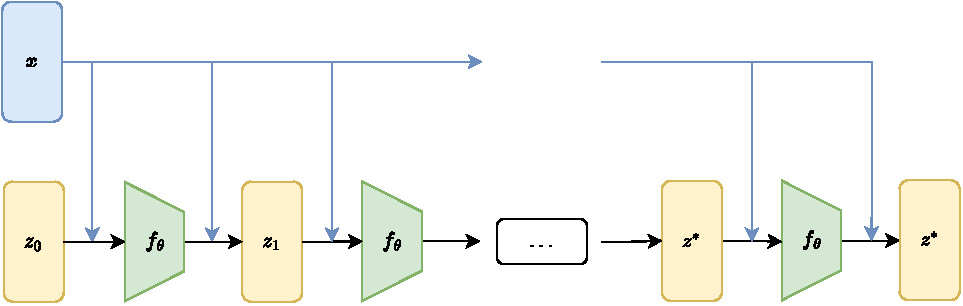
\includegraphics[width=0.9\textwidth]{../figures/deep_equilibrium_models/model_architecture.pdf}
  \caption{\textbf{Discrete DEQ Formulation}: Discrete DEQ Block where the input $x$ is injected at every iteration till the system (with initial state $z_0$) converges to a steady $\zstar$.}
  \label{fig:model_architecture_discrete_deq}
\end{figure}

Deep Equilibrium Networks (DEQs)~\citep{bai_deep_2019} are implicit models where the output space represents a steady-state solution. Intuitively, this represents infinitely deep neural networks with input injection, i.e., an infinite composition of explicit layers $z_{n + 1} = f_\theta(z_n, x)$ with $z_0 = 0$ and $n \rightarrow \infty$. In practice, it is equivalent to evaluating a dynamical system until it reaches a steady state $\zstar = f_\theta(\zstar, x)$.

% \citet{bai_deep_2019, bai_multiscale_2020} perform nonlinear fixed point iterations of the discrete dynamical system using Broyden's method~\citep{broyden1965class, bai_multiscale_2020} to reach this steady-state solution. 

Evaluating DEQs requires solving a steady-state equation involving multiple evaluations of the explicit layer slowing down the forward pass. However, driving the solution to steady-state makes the backward pass very efficient~\citep{johnson2012notes} (See \Cref{sec:sensitivity_analysis_ssproblems}). Despite a potentially infinite number of evaluations of $f_\theta$ in the forward pass, backpropagation only requires solving a linear equation.

\subsection{Nonlinear Solvers}
\label{subsec:nonlinear_solvers_deqs}

In this section, we will exclusively discuss Nonlinear Solvers for solving large steady state problems (i.e., systems with thousands of states).

\subsubsection{Broyden's Method}
\label{subsubsec:broyden_method}

Newton's method is a widely used iterative method for solving nonlinear systems of equations. It is an iterative method that uses the Jacobian matrix to update the solution vector in each iteration.
%
\begin{equation}
  x^{(k+1)} = x^{(k)} - \left( \frac{\partial \func{f}{x^{(k)}}}{\partial x} \right)^{-1} \func{f}{x^{(k)}} \label{eq:newton_method}
\end{equation}
%
However, computing the Jacobian matrix is computationally expensive (cubic time complexity) and memory-wise inefficient. Broyden's method~\citep{broyden1965class} is a quasi-Newton method that approximates the Jacobian matrix using the updates to the solution vector from previous iterations. Specifically, let $f(x)$ be a nonlinear function of the vector $x$, and let $x^{(k)}$ denote the solution vector at the $k$-th iteration. The approximation to the inverse of the Jacobian matrix at iteration $k$ is given by:
%
\begin{equation}
  B^{(k)} = B^{(k-1)} + \left(\frac{\Delta x^{(k)} - B^{(k - 1)} \Delta f^{(k)}}{\Delta x^{(k)^T} B^{(k - 1)} \Delta f^{(k)}}\right) \left(\Delta x^{(k)^T} B^{(k - 1)}\right)
\end{equation}
%
where $\Delta x^{(k)} = x^{(k)} - x^{(k-1)}$ is the step vector, and $\Delta f^{(k)} = \func{f}{x^{(k)}} - \func{f}{x^{(k-1)}}$ is the difference in the function values at the current and previous iterations. $B^{(k-1)}$ is the approximation to the Jacobian matrix at the previous iteration.

The solution vector at the $k$-th iteration is then updated using the following equation:
%
\begin{equation}
  x^{(k+1)} = x^{(k)} - B^{(k)}f(x^{(k)})
\end{equation}
%
Broyden's method has several advantages over Newton's method, including a lower computational cost per iteration, making it feasible for solving large nonlinear system of equations (like deep equilibrium models).

\subsubsection{Anderson Acceleration}
\label{subsubsec:anderson_acceleration}


\todo{verify the equations once}

Anderson acceleration~\citep{anderson1965iterative} is an iterative method for solving steady state problems of the form $f(x) = x$ that uses a combination of previous iterates to improve the convergence rate of fixed-point iterations. Define the residual $g(x) = f(x) - x$. For notational brevity let, $f^{(k)} =  \func{f}{x^{(k)}}$ and $g^{(k)} = \func{g}{x^{(k)}}$. The basic idea of Anderson acceleration is to construct a sequence $\left\{x^{(0)}, x^{(1)}, x^{(2)}, \ldots, x^{(K)}\right\}$ to accelerate the convergence of a fixed-point sequence. Given an initial guess $x^{(0)}$ and an integer mixing parameter $m \geq 1$, this method performs the following for each iteration $k$:
%
\begin{enumerate}
  \item Compute $m^{(k)} \leftarrow \funct{min}{m, k}$
  \item Let, $G^{(k)} \leftarrow \left[ g^{(k - m^{(k)})} \ldots g^{(k)} \right]$
  \item Let, $A^{(k)} \leftarrow \left\{ \alpha = \left( \alpha_0, \ldots, \alpha_{m^{(k)}} \right) \in \mathbb{R}^{m^{(k)} + 1} : \sum_{i = 0}^{m^{(k)}} \alpha_i = 1 \right\}$
  \item $\alpha^{(k)} \leftarrow \underset{\alpha \in A^{(k)}}{\texttt{argmin}} \left\| G^{(k)} \alpha \right\|_2$
  \item $x^{(k+1)} \leftarrow \sum_{i = 0}^{m^{(k)}} \alpha^{(k)}_i f^{(k - m^{(k)} + i)}$
\end{enumerate}
%
Anderson acceleration can be very effective for accelerating the convergence of fixed-point iterations for nonlinear problems, especially for problems with slow convergence or oscillatory behavior.

\subsubsection{Limited Memory Broyden's Method}
\label{subsec:limited_memory_broyden}

As described in \Cref{subsubsec:broyden_method}, we can avoid the computational complexity of inverting a Jacobian Matrix by using Broyden's method. However, as pointed out in \citet{bai_multiscale_2020}, even storing the Broyden matrix $B$ for a Nonlinear function $g_\theta: R^{32 \times 32 \times 80} \mapsto R^{32 \times 32 \times 80}$ requires nearly $25GB$ of storage. To circumvent this issue \citet{bai_multiscale_2020} propose a limited memory variant of Broyden's method. The idea is to write the low rank approximation matrix of the inverted jacobian $J^{-1}_{g_\theta}$ ($B$) as the sum of low rank updates:
%
\begin{align}
  B^{(i + 1)}     & = B^{(0)} + \sum_{k = i}^{i + 1} \mathbf{u}^{(k)} \mathbf{v}^{(k)^T} \\
  B^{(i + 1)}     & = B^{(0)} + UV^T                                                     \\
  \texttt{where } & B^{(0)} = -I
\end{align}
%
$\mathbf{u}$ and $\mathbf{v}$ come from Sherman-Morrison Formula~\citep{sherman1950adjustment}. In the limited memory version, \citet{bai_multiscale_2020} store the last $m$ low-rank updates for $\mathbf{u}$ and $\mathbf{v}$, and use a first-in-first-out approach to update $U$ and $V$.

\subsection{Jacobian Free Newton-Krylov Methods (JNFK) for solving Linear Systems}
\label{subsec:newton_krylov_methods}


% \todo{\url{https://en.wikipedia.org/wiki/Generalized_minimal_residual_method}}

% \todo{\url{https://citeseerx.ist.psu.edu/doc/10.1.1.636.3743}}

JFNK Methods are used to solve Linear System of Equations without actually computing the Jacobian Matrix. These methods require the ability to compute matrix-vector products. As we will observe in \Cref{subsec:adjoint_equations_deqs}, ability to avoid the computation of the Jacobian matrix is crucial for large scale steady state problems. JNFK methods use Krylov subspace $K_j$ of dimension $k$ to solve linear equations of the form $A x = b$  where $A \in \mathbb{R}^{n \times n}$ is a sparse, non-symmetric matrix, $b \in \mathbb{R}^n$ is a known vector, and $x \in \mathbb{R}^n$ is the solution vector.
%
\begin{align}
  K_j                 & = \func{\texttt{span}}{r_0, Ar_0, A^2 r_0, \dots, A^{j-1} r_0}\label{eq:krylov_subspace} \\
  \texttt{where } r_0 & = b - A x_0
\end{align}
%
% \todo{chatgpt}
% % In this section, we will describe Generalized Minimal Residual Method (GMRES) a popular JNFK method, that approximates the solution of $Ax = b$ using $x_n \in K_n$ which minimizes the Euclidean norm of the residual $r_n = b - A x_n$.
% The Generalized Minimal Residual Method (GMRES) is a widely used JNFK method for solving large-scale linear systems of equations of the form $Ax=b$. GMRES is an iterative method that generates a sequence of approximate solutions $x_k \in K_k$, where $K_k$ is the Krylov subspace of dimension $k$. GMRES seeks to find the approximate solution $x_k$ that minimizes the Euclidean norm of the residual $r_k = b - Ax_k$ over the subspace $K_k$. Specifically, GMRES solves the minimization problem
% %
% \begin{equation}
%   \min_{x \in K_k} |b - Ax|_2,
% \end{equation}
% %
% where $| \cdot |2$ denotes the Euclidean norm. The solution $x_k$ is obtained using the Arnoldi iteration, which generates an orthogonal basis ${q_1, q_2, \dots, q{k+1}}$ for $K_{k+1}$ using the Arnoldi algorithm. The Arnoldi algorithm constructs the upper Hessenberg matrix $H_k \in \mathbb{R}^{(k+1) \times k}$ and the vector $q_{k+1}$ such that

% \begin{equation}
%   AQ_k = Q_{k+1} H_k,
% \end{equation}

% where $Q_k = [q_1, q_2, \dots, q_k]$ and $Q_{k+1} = [q_1, q_2, \dots, q_{k+1}]$. The solution $x_k$ is then obtained by solving the least-squares problem

% \begin{equation}
%   \min_{y \in \mathbb{R}^k} | \beta e_1 - H_k y |_2,
% \end{equation}

% where $\beta = |b|_2$ and $e_1$ is the first standard basis vector. The approximate solution is then given by

% \begin{equation}
%   x_k = Q_k y_k.
% \end{equation}

% GMRES is known to converge for a wide range of problems and is particularly effective for large-scale, sparse linear systems. However, it may require a large number of iterations to achieve convergence, and each iteration requires solving a linear system, which can be computationally expensive. Additionally, GMRES can be sensitive to the choice of preconditioner, which is used to improve the convergence rate of the algorithm.


\subsection{Adjoint Equations}
\label{subsec:adjoint_equations_deqs}

In \Cref{sec:sensitivity_analysis_ssproblems}, we derived the following linear system of equations:
%
\begin{equation}
  \left( I - \frac{\partial \func{f_\theta}{\zstar}}{\partial \zstar} \right)^T \times \lambda = \left(\frac{\partial \func{g}{\zstar, \theta}}{\partial \zstar}\right)^T
\end{equation}
%
For DEQs, the state space is too large to compute the entire jacobian matrix $\frac{\partial \func{f_\theta}{\zstar}}{\partial \zstar}$. Instead of computing $ A = \left( I - \frac{\partial \func{f_\theta}{\zstar}}{\partial \zstar} \right)^T $, we can use Matrix-Free Methods discussed in \Cref{subsec:newton_krylov_methods} to solve \Cref{eq:ss_lambda_linear}. To use JFNK solvers we need to be efficiently compute:
%
\begin{align}
  A \times \lambda & = \lambda - \left( \frac{\partial \func{f_\theta}{\zstar}}{\partial \zstar} \right)^T  \times \lambda   \\
                   & = \lambda - \left( \lambda^T \times  \frac{\partial \func{f_\theta}{\zstar}}{\partial \zstar} \right)^T
\end{align}
%
The second term is the Vector-Jacobian Product (VJP) which can be efficiently computed by any reverse-mode automatic differentiation framework (without constructing the entire Jacobian). Additionally, in \Cref{eq:ss_total_gradient} we can compute $\lambda^T \times \frac{\partial \func{f_\theta}{\zstar}}{\partial \theta}$ using the VJP trick using any reverse-mode automatic differentiation framework.

% \section{Convergence Criteria}
% \label{sec:ssproblem_convergence_criteria}

% \todo{\url{https://docs.sciml.ai/NonlinearSolve/stable/basics/TerminationCondition/}}

\section{Common Applications of DEQs}
\label{sec:common_applications_deqs}

\section{Accelerating DEQs}
\label{sec:accelerating_deqs}

DEQs share the benefits of implicit neural networks in reducing the memory requirements for training. Specifically, DEQs reduce the memory complexity from $\bigO{SL}$ where $S$ is the dimensions of the output and $L$ is the number of layers to $\bigO{S}$. However, a major concern is the high cost of forward pass which requires solving a steady state problem. An expensive forward pass is not only a bottleneck for training but also hinders deployment, that rely on fast inference. In this section, we discuss some prior works that accelerate the training and inference of DEQs.

\subsection{Jacobian Regularization of DEQs}
\label{subsec:jacobian_regularization_deqs}

\citet{bai2021stabilizing}

\subsection{Jacobian-Free Backpropagation}
\label{subsec:jacobian_free_backpropagation}

\citet{fung2022jfb}

\subsection{Neural Deep Equilibrium Solvers}
\label{subsec:neural_deep_equilibrium_solvers}

\citet{bai2021neural}
